% --------------------------------------------------------------------------------
% Student guideline for the final year dissertation using LaTeX2e
% Alexandra Bonnici
% Department of Systems and Control
% 13th September 2017

\documentclass[12pt, oneside]{Thesis}

% --------------------------------------------------------------------------------
% Some useful packages
% You may add/remove any packages as you deem fit,
% Recommended packages which are recommended are marked by [R] in the comment
% --------------------------------------------------------------------------------

% font options & general typesetting
\usepackage{microtype}            % some refinements over the general appearance of text
\usepackage{eqparbox}             % ensures that blocks of text occupy the same space

% for figures
\usepackage[]{graphicx}     %  [R] to use graphics
\usepackage{subfigure}            %  [R] to make subfigures
\usepackage{epstopdf}             %  [R] adds eps support in the graphics package
\usepackage{wrapfig}              %  to allow text to wrap around figures


% for tables
\usepackage[table]{xcolor}
\usepackage{multirow,bigstrut}    % to have tables with merged rows
\usepackage{array, booktabs}      %  [R] for good looking tables
\usepackage{longtable}            % to create tables that span more than one page
\usepackage{adjustbox}            % so that long tables fit within the page
\usepackage{rotating}             % adds support to rotate pages

% to write nice mathematical equations
\usepackage{mathtools}            %  [R] some mathematical tools
\usepackage{amsmath}		      %  [R] to write math formulas easily
\usepackage{amssymb}              %  [R] for maths symbols
\usepackage{amsthm}               % for the typesetting of theorems
\usepackage{esvect}               % to make vector arrows
\usepackage{bm}                   % to make bold maths symbols

\usepackage{xfrac}                % [R] to make in-text fractions

% more symbols
\usepackage{pifont}               % Postscript standard Symbol and Dingbats fonts
\usepackage{gensymb}              % generic symbols fonts
\usepackage{stackrel}             % to stack things on top of each other

% to include urls
\usepackage{url}                  % to write urls

% to typeset pseudo code algorithms and source codes
\usepackage{algorithm}            % to type set algorithms as pseudo code
\usepackage{algpseudocode}        % more layout options for algorithm pseudo code
\usepackage{listings}             % to add non-formatted text e.g. source code

\usepackage{todonotes}
\lstdefinestyle{myLuastyle}
{
  language         = {[5.2]Lua},
  basicstyle       = \ttfamily,
  showstringspaces = false,
  upquote          = true,
}
\lstset{style=myLuastyle}
% to typeset theorems, lemmas and definitions
\newtheorem{theorem}{Theorem}[chapter]
\newtheorem{lemma}{Lemma}
\newtheorem{definition}{Definition}

\newcommand{\paratitle}[1]{\underline{\textbf{\emph{#1}}}}
\newcommand{\keyword}[1]{\textcolor{red}{\emph{#1}}}
% \usepackage{enumitem}

% --------------------------------------------------------------------------------
% Information relevant to your dissertation.
% Substitute with your own name, supervisor and title details.
%--------------------------------------------------------------------------------

\thesistitle{LuaJIT Internals \\ {\large v2.1.0-beta3 (1 May 2017)}} % title
\authors{A. \textsc{Bloch} and L. \textsc{Deniau}}	% your name
\keywords{LuaJIT, technical documentation}         	% keywords
%\department{}                						% department name
%\Udegree{}
\subject{LuaJIT Internals}
%\UNIVERSITY{}
%\faculty{Faculty of Engineering}

%\newif\ifHaveACosupervisor
% toggle the comment on the true/false lines as appropriate
%\HaveACosupervisortrue
%\HaveACosupervisorfalse

%--------------------------------------------------------------------------------
% Creates the PDF meta-data (for the electronic version of your dissertation).
% There is no need to modify this information
%--------------------------------------------------------------------------------
\hypersetup{urlcolor=blue,%
		    linkcolor=blue,%
            citecolor=blue,%
            colorlinks=true,%
            hypertexnames=true}

\hypersetup{pdftitle={\ttitle}}
\hypersetup{pdfsubject=\subjectname}
\hypersetup{pdfauthor=\authornames}
\hypersetup{pdfkeywords=\keywordnames}

%--------------------------------------------------------------------------------
% Creates the title page (typesetting is taken care of and details are as above)
%--------------------------------------------------------------------------------
\title{\ttitle}

%--------------------------------------------------------------------------------
% Creates the glossaries pages and index pages
%--------------------------------------------------------------------------------
\makeglossaries
\makeindex

%--------------------------------------------------------------------------------
% The actual start of the dissertation
%--------------------------------------------------------------------------------
\begin{document}

\frontmatter            % sets page numbers of the first few pages to roman
\setstretch{1.3}        % ensures a one-and-a-half line spacing
\fancyhead{}            % clears the headers
\rhead{\thepage}        % sets the top right header to the page number
\lhead{}                % ensures that the top left header remains empty
\pagestyle{fancy}     	% uses the "fancy" page style (adds the line at top)


%--------------------------------------------------------------------------------
% Prints out the title page
%--------------------------------------------------------------------------------
\begin{titlepage}

\flushleft{\textsc{\large European Organization for Nuclear Research -- CERN}\\
\large Beams Department --  Accelerators Beams Physics Group}

\vspace{2cm}
\begin{center}
\linespread{1.3}\huge \bfseries \ttitle
\end{center}
\vspace{2cm}
\begin{center}
by \\[1cm]
\authornames\\[5cm]
\large Dissertation open to the community of LuaJIT \\[1cm]
\vfill
\end{center}

\end{titlepage}


% -------------------------------------------------------------------------------
% Prints out the copyright page (you do not need to modify this)
%--------------------------------------------------------------------------------
\clearpage
\Copyright{

\addtocontents{toc}{\vspace{1em}}
\vspace{2cm}

\begin{enumerate}
\item Copyright in text of this dissertation rests with the Author. Copies (by any process) either in full, or of extracts may be made only in accordance with regulations held by the Library of the University of Malta. Details may be obtained from the Librarian. This page must form part of any such copies made. Further copies (by any process) made in accordance with such instructions may not be made without the permission (in writing) of the Author.
\item Ownership of the right over any original intellectual property which may be contained in or derived from this dissertation is vested in the University of Malta and may not be made available for use by third parties without the written permission of the University, which will prescribe the terms and conditions of any such agreement.
\end{enumerate}}

%--------------------------------------------------------------------------------
% Prints out the abstract
% You will need to change the text in the file to reflect your own abstract
%--------------------------------------------------------------------------------
\clearpage
\addtotoc{Abstract}
\abstract{\addtocontents{toc}{\vspace{1em}}

TODO
}


%--------------------------------------------------------------------------------
% Prints out the acknowledgements page
% You will need to change the text to reflect your own acknowledgements
%--------------------------------------------------------------------------------
\clearpage
\setstretch{1.3}

\acknowledgements{\addtocontents{toc}{\vspace{1em}}
I would like to thank Mike Pall for his commitment for the LuaJIT Project
} 

%--------------------------------------------------------------------------------
% Prints out the list of contents, figures and tables
% You don't have to modify any of this
%--------------------------------------------------------------------------------
\clearpage
\pagestyle{fancy}

\lhead{\emph{Contents}}
\tableofcontents

\lhead{\emph{List of Figures}}
\listoffigures

\lhead{\emph{List of Tables}}
\listoftables

%--------------------------------------------------------------------------------
% Prints out the list of acronyms
% No changes will be necessary if used properly within text
%--------------------------------------------------------------------------------
\clearpage
\setglossarystyle{altlist}
\printglossary[type=\acronymtype, title=List of Acronyms, toctitle=List of Acronyms]

%--------------------------------------------------------------------------------
% Prints out the list of symbols
% No changes will be necessary if used properly within text, comment if not relevant
%--------------------------------------------------------------------------------

\clearpage
\setglossarystyle{list}
\printglossary[title=List of Symbols,toctitle=List of Symbols]


%--------------------------------------------------------------------------------
% Prints out the chapter contents
%--------------------------------------------------------------------------------

\mainmatter
\pagestyle{fancy}

\clearpage
\chapter{Introduction}
\label{Chapt:Introduction}
\lhead{Chapter \thechapter. \emph{Introduction}}
\input{./Chapters/Introduction}

% \clearpage
% \chapter{Overview}
% \label{Chapt:Overview}
% \lhead{Chapter \thechapter. \emph{Overview}}
% %!TEX root = ../FYP_Dissertation.tex
TODO:\\
General introduction on luaJIT (tracing jit).\\
Write a paragraph per Part (Lexer, Parser, VM, JIT).\\
Add a schema on how things are connected(simalar of the one in  Laurent's slide).


\part{Overview}
\label{Part:Overview}

  \chapter{Files hierarchy}
  \label{Chapt:files}
  \lhead{Chapter \thechapter. \emph{Files hierarchy}}
  %!TEX root = ../FYP_Dissertation.tex
\paratitle{dynasm/*:}\\
All files in this folder correspond to the Dynamic Assembler (see Apendix \ref{Apendix:DynASM})\\
\paratitle{dynasm/dasm\_*.h:}\\
DynASM encoding engine for a specific architecture.\\
\paratitle{dynasm/dasm\_*.lua:}\\{}
DynASM lua module for a specific architecture.\\
\paratitle{dynasm/dynasm.lua:}\\
DynASM mechanism main source file.\\
\paratitle{src/host/*:}\\
The files in this directory are only used during the build process of LuaJIT.
For cross-compilation, they must be executed on the host, not on the target.\\
\paratitle{src/host/buildvm.c:}\\
\paratitle{src/host/buildvm.h:}\\
\paratitle{src/host/buildvm\_asm.c:}\\
\paratitle{src/host/buildvm\_fold.c:}\\
\paratitle{src/host/buildvm\_lib.c:}\\
\paratitle{src/host/buildvm\_libbc.h:}\\
\paratitle{src/host/buildvm\_peobj.c:}\\
\paratitle{src/host/genlibbc.lua:}\\
\paratitle{src/host/genminilua.lua:}\\
\paratitle{src/host/minilua.c:}\\
Minimal copy of Lua 5.1 used to build LuaJIT.\\
\paratitle{src/jit/bc.lua:}\\
\paratitle{src/jit/bcsave.lua:}\\
Lua module used to save the bc of a source file.\\
\paratitle{src/jit/dis\_*.lua:}\\
LuaJIT disassembler module for a specific architecture, used as a help module by
the dumper mode to dump code of generated trace (See dump.lua).\\
\paratitle{src/jit/dump.lua:}\\
LuaJIT compiler dump module (see Chapter \ref{Chapt:Dump-mode}).\\
\paratitle{src/jit/p.lua:}\\
LuaJIT profiler (see Chapter \ref{Chapt:Profiler}).\\
\paratitle{src/jit/v.lua:}\\
LuaJIT verbose mode (see Chapter \ref{Chapt:Verbose}).\\
\paratitle{src/jit/zone.lua:}\\
This module implements a simple hierarchical zone model
(See \emph{zone} in Chapter \ref{Chapt:Profiler}).\\
\paratitle{src/lauxlib.h:}\\
Auxiliary library for the Lua/C API.\\
\paratitle{src/lib\_*.c:}\\
Implement a library with an interface available through lua code.\\
\paratitle{src/lib\_aux.c:}\\
\paratitle{src/lib\_aux.c:}\\
\paratitle{src/lib\_base.c:}\\
\paratitle{src/lib\_bit.c:}\\
\paratitle{src/lib\_debug.c:}\\
\paratitle{src/lib\_ffi.c:}\\
FFI library.\\
\paratitle{src/lib\_init.c:}\\
\paratitle{src/lib\_io.c:}\\
\paratitle{src/lib\_jit.c:}\\
\paratitle{src/lib\_math.c:}\\
\paratitle{src/lib\_os.c:}\\
\paratitle{src/lib\_package.c:}\\
\paratitle{src/lib\_string.c:}\\
\paratitle{src/lib\_table.c:}\\
\paratitle{src/lj\_alloc.[ch]:}\\
Bundled memory allocator.\\
\paratitle{src/lj\_api.c:}\\
Lua/c api (e.g. stack handling)\\
\paratitle{src/lj\_arch.h:}\\
\paratitle{src/lj\_asm.[ch]:}\\
Generic code for assembling a trace.\\
\paratitle{src/lj\_asm\_*.h:}\\
IR assembler, convert SSA IR into machine code for a specific architecture.\\
\paratitle{src/lj\_bc.[ch]:}\\
Bytecode instruction format.\\
\paratitle{src/lj\_bcdump.h:}\\
\paratitle{src/lj\_bcread.c:}\\
Bytecode reader to allow executing saved bc.\\
\paratitle{src/lj\_bcwrite.c:}\\
Bytecode writer to save bc.\\
\paratitle{src/lj\_buf.c:}\\
\paratitle{src/lj\_buf.h:}\\
\paratitle{src/lj\_carith.[ch]:}\\
C data arithmetic.\\
\paratitle{src/lj\_ccall.[ch]:}\\
FFI C call handling.\\
\paratitle{src/lj\_ccallback.[ch]:}\\
FFI C callback handling.\\
\paratitle{src/lj\_cconv.[ch]:}\\
C type conversions.\\
\paratitle{src/lj\_cdata.[ch]:}\\
C data management.\\
\paratitle{src/lj\_char.c:}\\
\paratitle{src/lj\_char.h:}\\
\paratitle{src/lj\_clib.[ch]:}\\
FFI C library loader.\\
\paratitle{src/lj\_cparse.[ch]:}\\
C declaration parser.\\
\paratitle{src/lj\_crecord.c:}\\
\paratitle{src/lj\_crecord.h:}\\
\paratitle{src/lj\_ctype.[ch]:}\\
C type management.\\
\paratitle{src/lj\_debug.c:}\\
\paratitle{src/lj\_debug.h:}\\
\paratitle{src/lj\_def.h:}\\
\paratitle{src/lj\_dispatch.c:}\\
\paratitle{src/lj\_dispatch.h:}\\
\paratitle{src/lj\_emit\_*.h:}\\
Instruction emitter for a specific architecture.\\
\paratitle{src/lj\_err.c:}\\
\paratitle{src/lj\_err.h:}\\
\paratitle{src/lj\_errmsg.h:}\\
\paratitle{src/lj\_ff.h:}\\
\paratitle{src/lj\_ffrecord.c:}\\
\paratitle{src/lj\_ffrecord.h:}\\
\paratitle{src/lj\_frame.h:}\\
\paratitle{src/lj\_func.[ch]:}\\
Function handling, prototype and upvalues.\\
\paratitle{src/lj\_gc.[ch]:}\\
Garbage collector implementation\\
\paratitle{src/lj\_gdbjit.c:}\\
\paratitle{src/lj\_gdbjit.h:}\\
\paratitle{src/lj\_ir.c:}\\
\paratitle{src/lj\_ir.h:}\\
\paratitle{src/lj\_ircall.h:}\\
\paratitle{src/lj\_jit.h:}\\
\paratitle{src/lj\_lex.c:}\\
Lexer (Lexical analyzer) for lua code.\\
\paratitle{src/lj\_lex.h:}\\
Main header file used during the lexer, parser and bcreader.\\
\paratitle{src/lj\_lib.c:}\\
\paratitle{src/lj\_lib.h:}\\
\paratitle{src/lj\_load.c:}\\
\paratitle{src/lj\_mcode.c:}\\
\paratitle{src/lj\_mcode.h:}\\
\paratitle{src/lj\_meta.c:}\\
\paratitle{src/lj\_meta.h:}\\
\paratitle{src/lj\_obj.c:}\\
\paratitle{src/lj\_obj.h:}\\
\paratitle{src/lj\_iropt.h:}\\
Common header for IR emitter and optimizations.\\
\paratitle{src/lj\_opt\_*.c:}\\
IR optimization implementation for a specific type of optimization.\\
\paratitle{src/lj\_parse.[ch]:}\\
Lua parser and bc generator\\
\paratitle{src/lj\_profile.c:}\\
\paratitle{src/lj\_profile.h:}\\
\paratitle{src/lj\_record.[ch]:}\\
Trace recorder converts bytecode into SSA IR.\\
\paratitle{src/lj\_snap.[ch]:}\\
Creates and handles trace snapshots.\\
\paratitle{src/lj\_state.c:}\\
\paratitle{src/lj\_state.h:}\\
\paratitle{src/lj\_str.[ch]:}\\
Internal String handling.\\
\paratitle{src/lj\_strfmt.c:}\\
\paratitle{src/lj\_strfmt.h:}\\
\paratitle{src/lj\_strfmt\_num.c:}\\
\paratitle{src/lj\_strscan.c:}\\
\paratitle{src/lj\_strscan.h:}\\
\paratitle{src/lj\_tab.[ch]:}\\
Lua table handling.
\paratitle{src/lj\_target.h:}\\
Generic definitions for target CPU.\\
\paratitle{src/lj\_target\_*.h:}\\
Definitions for target CPU for a specific architecture.\\
\paratitle{src/lj\_trace.[ch]:}\\
Trace management.\\
\paratitle{src/lj\_traceerr.h:}\\
\paratitle{src/lj\_udata.c:}\\
\paratitle{src/lj\_udata.h:}\\
\paratitle{src/lj\_vm.h:}\\
\paratitle{src/lj\_vmevent.c:}\\
\paratitle{src/lj\_vmevent.h:}\\
\paratitle{src/lj\_vmmath.c:}\\
\paratitle{src/ljamalg.c:}\\
LuaJIT core and libraries amalgamation (Used in amalg compilation target to generate better binaries).\\
\paratitle{src/lua.h:}\\
\paratitle{src/lua.hpp:}\\
\paratitle{src/luaconf.h:}\\
\paratitle{src/luajit.c:}\\
\paratitle{src/luajit.h:}\\
\paratitle{src/lualib.h:}\\
\paratitle{src/msvcbuild.bat:}\\
\paratitle{src/ps4build.bat:}\\
\paratitle{src/psvitabuild.bat:}\\
\paratitle{src/vm\_*.dasc:}\\
Virtual Machine written using DynASM for a specific architecture (see Chapter \ref{Chapt:DynASM} for DynASM and Part \ref{Part:VM} for the VM)\\
\paratitle{src/xb1build.bat:}\\
\paratitle{src/xedkbuild.bat:}\\

  \chapter{Major data structure}
  \label{Chapt:ds}

  \chapter{Tools}
  \label{Chapt:Tools}
  \lhead{Chapter \thechapter. \emph{Tools}}
  %!TEX root = ../FYP_Dissertation.tex
\section{Verbose mode}
\label{Sec:Verbose}

This module shows verbose information about the progress of the
JIT compiler. It prints one line for each generated trace. This module
is useful to see which code has been compiled or where the compiler
punts and falls back to the interpreter.

Example usage:

\begin{lstlisting}
  luajit -jv -e "for i=1,1000 do for j=1,1000 do end end"
  luajit -jv=myapp.out myapp.lua
\end{lstlisting}
To redirect the output to a file, pass a
filename as an argument (use '-' for stdout) or set the environment
variable LUAJIT\_VERBOSEFILE. The file is overwritten every time the
module is started.

The output from the second example could look like this:

\begin{center}
[TRACE   1 myapp.lua:1 loop]

[TRACE   2 (1/3) myapp.lua:1 $->$ 1]
\end{center}

The first number in each line is the internal trace number. Next are
the file name ('myapp.lua') and the line number (':1') where the
trace has started. Side traces also show the parent trace number and
the exit number where they are attached to in parentheses ('(1/3)').
An arrow at the end shows where the trace links to ('$->$ 1'), unless
it loops to itself.

In this case the inner loop gets hot and is traced first, generating
a root trace. Then the last exit from the 1st trace gets hot, too,
and triggers generation of the 2nd trace. The side trace follows the
path along the outer loop and \textit{around} the inner loop, back to its
start, and then links to the 1st trace.

Aborted traces are shown like this:
\begin{center}
[TRACE --- foo.lua:44 -- leaving loop in root trace at foo:lua:50]
\end{center}

Trace aborts are quite common, even in programs which
can be fully compiled. The compiler may retry several times until it
finds a suitable trace. This doesn't work with features that are
not-yet-implemented (NYI error messages). The VM simply falls back to the
interpreter. This may not matter at all if the particular trace is not very high
up in the CPU usage profile, plus the interpreter is quite fast, too.

\section{Profiler}
\label{Sec:Profiler}

This module is a simple command line interface to the built-in
low-overhead profiler of LuaJIT. The lower-level API of the profiler
is accessible via the "jit.profile" module or the luaJIT\_profile\_* C API.

Example usage:
\begin{lstlisting}
  luajit -jp myapp.lua
  luajit -jp=s myapp.lua
  luajit -jp=-s myapp.lua
  luajit -jp=vl myapp.lua
  luajit -jp=G,profile.txt myapp.lua
\end{lstlisting}
The following dump features are available:
 \begin{itemize}%[label={--}]
  \item \textbf{f} - Shows function name (Default mode).
  \item \textbf{F} - Shows function name with module prepend.
  \item \textbf{l} - Shows line granularity ('module':'line').
  \item \textbf{\textless number\textgreater} - Stack dump depth (callee\textless caller - Default: 1)
  \item \textbf{-\textless number\textgreater} - Inverse stack dump depth (caller\textgreater callee).
  \item \textbf{s} - Split stack dump after first stack level. Implies $\mid depth\mid$
  \textgreater= 2.
  \item \textbf{p} - Show full path for module names.
  \item \textbf{v} - Show VM states (See bellow).
  \item \textbf{z} - Show zones (See bellow).
  \item \textbf{r} - Show raw sample counts (Default: percentages).
  \item \textbf{a} - Annotate excerpts from source code files.
  \item \textbf{A} - Annotate complete source code files.
  \item \textbf{G} - Produce raw output suitable for graphical tools (See bellow).
  \item \textbf{m\textless number\textgreater} - Minimum sample percentage to be shown (Default: 3).
  \item \textbf{i\textless number\textgreater} - Sampling interval in milliseconds (Default: 10).
 \end{itemize}

 Many of those options can be activated at ones.\\

\paratitle{VM states:}\\
This options allows to shows the time spent in which state of the VM.
States can be of the following types :

\{Compiled - Interpreted - C code - Garbage Collector - JIT Compiler\} \\

\paratitle{Zone:}\\
statistics can be grouped in user defined zone. Bellow is an example a such a
definition.
\begin{lstlisting}
    local zone = require("jit.zone")
    zone("MyZone")
      -- Lua code here
    zone()
\end{lstlisting}

\paratitle{Graphical tools:}\\
This option can be used to graphically show the dump in a nice image format
(see Appendix \ref{Apendix:fl})

\section{Dump mode}
\label{Sec:Dump-mode}

This module can be used to debug the JIT compiler itself. It dumps the
code representations and structures used in various compiler stages.

Example usage:
\begin{lstlisting}
  luajit -jdump -e "
    local x=0
    for i=1,1e6 do x=x+i end
    print(x)
  "
  luajit -jdump=im -e "
    for i=1,1000 do
      for j=1,1000 do end
    end
  " | less -R
  luajit -jdump=is myapp.lua | less -R
  luajit -jdump=-b myapp.lua
  luajit -jdump=+aH,myapp.html myapp.lua
  luajit -jdump=ixT,myapp.dump myapp.lua
\end{lstlisting}
The first argument specifies the dump mode. The second argument gives
the output file name. Default output is to stdout, unless the environment
variable LUAJIT\_DUMPFILE is set. The file is overwritten every time the
module is started. Different features can be turned on or off with the dump mode.
If the mode starts with a '+', the following features are added to the default
set of features; a '-' removes them. Otherwise the features are replaced.\\
The following dump features are available (* marks the default):

\begin{itemize}
  \item \textbf{t *} - Print a line for each started, ended or aborted trace (see also -jv).
  \item \textbf{b *} - Dump the traced bytecode.
  \item \textbf{i *} - Dump the IR (intermediate representation).
  \item \textbf{r} - Augment the IR with register/stack slots.
  \item \textbf{s} - Dump the snapshot map.
  \item \textbf{m *} - Dump the generated machine code.
  \item \textbf{x} - Print each taken trace exit.
  \item \textbf{X} - Print each taken trace exit and the contents of all registers.
  \item \textbf{a} - Print the IR of aborted traces, too.
\end{itemize}
The output format can be set with the following characters:
\begin{itemize}
   \item \textbf{T} - Plain text output.
   \item \textbf{A} - ANSI-colored text output
   \item \textbf{H} - Colorized HTML + CSS output.
\end{itemize}
The default output format is plain text. It's set to ANSI-colored text
if the COLORTERM variable is set.

\part{Interpreter}
\label{Part:Interpreter}

  \chapter{Lexer}
  \label{Chapt:Lexer}

  \chapter{Parser}
  \label{Chapt:Parser}

  \chapter{Bytecode emitter}
  \label{Chapt:BC}

\part{Virtual Machine}
\label{Part:VM}

  \chapter{Bytecode interpreter}
  \label{Chapt:BI}
  %!TEX root = ../FYP_Dissertation.tex
Most a the VM mechanism is written using the DynASM syntax. To get a better
understanding of the underlining technology see Appendix \ref{Apendix:DynASM}.

The low-level VM code written for each architecture using this assembler can be
found in \emph{vm\_(target).dasc} files. It is mainly composed of the switch
case that generate the assembly code for each byte code, but it also contains
code for other part that requires low level implementation such as the
stack unwinding or the implementation of the fast path of asm fast library functions
(see section \ref{Subsec:ffunc} for more).

  \chapter{Foreign function interface}
  \label{Chapt:FFI}

  \chapter{Library function interface}
  \label{Chapt:LFI}

\part{JIT}
\label{Part:JIT}

  \chapter{Trace record}
  \label{Chapt:TR}
  %!TEX root = ../FYP_Dissertation.tex

%===============================================================================
% Hot path detection
%===============================================================================

\section{Hot path detection}
\label{Sec:hot-path}

LuaJIT does trace compilation. For that, it needs to detect that a certain
portion of the code gets hot and compile it as a trace. Two types of trace entry
are detected, loops and function. In the vm (See Part \ref{Part:VM}) each
traceable loop-like or call-like BC (bytecode) decrement a low-overhead profile
counter that is at the hashed PC (program counter) position of a 64-entries table.
When the counter underflows, it start recording. Bellow is the call order that
trigger a recording depending of the bytecode. This counter table being small
and collision being ignored false positive may occur.
It must be noted that LuaJIT perform a natural-loop first (NLF) region selection.
This can be noted in two ways. First, when the BC is a loop the counters are
decremented twice as fast as for function call. Second, In most cases, if a
parent trace hit an inner loop, the parent trace is aborted.

\paratitle{Loops:}

\begin{itemize}
	\item \emph{hotloop} : hash the pc, decrement the corresponding counter and
jmp to vm\_hotloop if it underflows (vm\_(arch).dasc).
	\item \emph{vm\_hotloop} : Prepare the stack and call lj\_trace\_hot.
	\item \emph{lj\_trace\_hot} : start recording a trace (lj\_trace.c).
\end{itemize}

\paratitle{Functions:}

\begin{itemize}
	\item \emph{hotcall} : hash the pc, decrement the corresponding counter and
jmp to vm\_hotcall if it underflows (vm\_(arch).dasc).
	\item \emph{vm\_hotcall} : Prepare the stack and call lj\_dispatch\_call.
	\item \emph{lj\_dispatch\_call} : perform initialization
	and call \emph{lj\_trace\_hot} that start recording a trace (lj\_dispatch.c).
\end{itemize}

\emph{lj\_trace\_hot} start the recording of a parent trace by changing
\emph{J$->$state} to \emph{LJ\_TRACE\_START}, starting the recorder state
machine, described in the next section.


%===============================================================================
% Recorder state machine
%===============================================================================

\section{Recorder state machine}
\label{Sec:recorder-state-machine}

Recording is the fact of executing the bytecode while remembering dynamic
data/type and generating on the fly the IR specialized for this recording. In
doing so, the control flow is flattened meaning that only taken branch are
recorded and function call are inlined. The code responsible for that lie in, the
\emph{lj\_trace.c} file for the state machine presented bellow and the helper
functions, the \emph{lj\_record.c} for most of the bytecode recording,
the \emph{lj\_ffrecord.c} for the data of fast function call and
\emph{lj\_crecord.c} for the cdata operations.

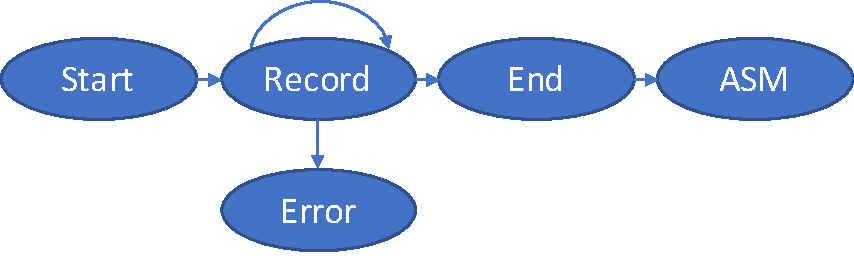
\includegraphics[width=\textwidth]{./Images/FSM.pdf}

\begin{table}[H]
\centering
\caption{Library Macro definitions}
\label{tab:library-macro}
\begin{tabularx}{\textwidth}{|c|X|}
\hline
\multicolumn{1}{|c|}{Macro}          & \multicolumn{1}{c|}{Description}                     \\\hline
Start                   &
  \begin{tabular}[c]{@{}l@{}}
  Call trace\_start that perform jit\_State setup and \\allocations.
  Change state to LJ\_TRACE\_RECORD.
  \end{tabular}                                                                             \\\hline
Record                  & Recording in progress. It loop over the
	lj\_record\_ins function, which is a huge switch case that record a specific
  bytecode instruction and generate the corresponding specialized IR code of the
  BC before execution. It is executed inside a pcall and jump to the
  \emph{Error} state if a lua exception is thrown. \\\hline%
End                     &
  End of recording. It applies optimizations on the IR (see Chapter \ref{Chapt:TO}).        \\\hline
ASM                     &
	Assemble the trace and call trace\_stop to patch the BC (see Chapter \ref{Chapt:TA}).     \\\hline
Error                   &
	Abort the recording of the current trace, perform state cleanup, penalize the
	corresponding hot BC or apply blacklisting (see Section \ref{Sec:abort})                  \\\hline
\end{tabularx}
\end{table}

%===============================================================================
% Abortion and blacklisting
%===============================================================================

\section{Abortion and blacklisting}
\label{Sec:abort}

There exist multiple reason that might cause a recording to abort. Such reason
could be that the unroll limit is reached, that the trace is too long, that the
jit is disable for a specific function or many other. (see \emph{lj\_traceerr.h}
for the list of possible abort messages). To trigger an abortion, a lua error is
thrown during the recording which transition the recorder state machine to the
\emph{LJ\_TRACE\_ERR} state. Then, the \emph{penalty\_pc} function is called on
the hot bytecode that triggered the recording. The penalty mechanism consist of
a 64-entry table, where each entry is a structure containing the exact PC of the
penalized bytecode, the penalty value, and the reason of the abortion. The
\emph{penaltyslot} variable is a round-robin index inside the table indicating
the next entry to use if a new bytecode needs to be penalized. It as to be noted
that on the contrary of the hotcount mechanisme, here the full PC is used to
identify a slot making it free of false positive. However, since the entry is
only 64 entry, penalized bytecode can easily be forgotten in a big code base.
If the penalty for a given bytecode exceeds a threshold then the hot bytecode
responsible for starting the recording gets blacklisted. It meaning that this
bytecode can never become hot again to start a recording and that if this
bytecode try to be recorded inside another trace, this trace get aborted too
(in most cases). A blacklisted bytecode is never whitelisted by the system.

%===============================================================================
% Intermediate representation
%===============================================================================

\section{Intermediate representation}
\label{Sec:IR}

% IR:
% ----
% - SSA (Static single assignment) based (cf : https://www.wikiwand.com/en/Static_single_assignment_form)
% - Data-flow for loops is represented using PHI-instructions.
% - Control-flow is always implicit.
% - operands are 16 bit references
% - implemented with a bidirectionally growable array
% - Skip-list chains: The IR is threaded with segregated, per-opcode
%   skip-list chains. The links are stored in a multi-purpose 16 bit
%   field in the instruction. This facilitates low-overhead lookup
%   for CSE, DSE and alias analysis. Back-linking enables short-cut
%   searches (average overhead is less than 1 lookup). Incremental
%   build-up is trivial. No hashes, no sets, no complex updates.
% - a single High-level IR across all optimization stage.
% - Trace IR code is represented as an array in memory.
% - The array includes two different things: instructions and constants.
% - Instructions are stored at "upwards" indices 0,1,2,... ( > 0x8000 )
% - Constants are stored at "downwards" indices -1,-2,-3,... ( < 0x8000 )
% - References to array elements are "biased" by adding 0x8000.
% - ir reference are index in the ir array.
% - Every instruction has an output data type.
% - IR constants are interned and can be compared for equality only by looking at their references.
% - Guarded assertions have a dual purpose
%   - They provide an assertion about their operands.
%   - They are emitted by the backend as branching comparisons,
%     - true ->  fall-through path.
%     - false ->  outcome exits the trace and restores the state using last snapshot.

% -- IR instruction format (64 bit).
% --
% --    16      16     8   8   8   8
% -- +-------+-------+---+---+---+---+
% -- |  op1  |  op2  | t | o | r | s |
% -- +-------+-------+---+---+---+---+
% -- |  op12/i/gco32 |   ot  | prev  | (alternative fields in union)
% -- +-------+-------+---+---+---+---+
% -- |  TValue/gco64                 | (2nd IR slot for 64 bit constants)
% -- +---------------+-------+-------+
% --        32           16      16
% --
% -- prev is only valid prior to register allocation and then reused for r + s.
% --
% -- t    : type
% -- o    : opcode
% -- r    : register allocation
% -- s    : spill slot
% -- prev : chain of instruction of same opcode


%===============================================================================
% Snapshots
%===============================================================================

\section{Snapshots}
\label{Sec:snap}

Snapshot is an important mechanism used in trace compilation. The VM should
always be in a consistent state, meaning that all updates should respect the
original language semantics. However, to perform some trace optimization
(e.g. sinking optimization) this consistency is not respected. Instead
modification that should have occurred during a trace is recorded inside the
snapshots and those modification are replayed at trace exit. The Snapshot
mechanism is implemented in the snap.[hc] files, and you can find the
\emph{SnapShot} data-structure in lj\_jit.h. For details about
Snapshot usages and implementation refer to section of the wiki on sinking
optimization \cite{luajit-sink} and a mail on the subject \cite{luajit-mail-1}.


  \chapter{Intermediate representation}
  \label{Chapt:IR}
  %!TEX root = ../FYP_Dissertation.tex


  \chapter{Trace manager}
  \label{Chapt:TM}
  %!TEX root = ../FYP_Dissertation.tex


  \chapter{Trace optimizer}
  \label{Chapt:TO}
  %!TEX root = ../FYP_Dissertation.tex

We can differentiate in the code, three types of optimizations.
First of all there are the optimizations present in the optimization engine.
They are implemented in the \emph{lj\_opt\_*.c} files and thus easy to spot out.
Those optimization are of two kind, global optimization that are run on the
entire IR at once at the end of the recording phase, during the
\emph{LJ\_TRACE\_END} state (See \ref{Subsec:opt-dce}, \ref{Subsec:opt-loop},
\ref{Subsec:opt-split}, \ref{Subsec:opt-sinking}) and the local optimizations
that are applied while recording a trace (See \ref{Subsec:narrowing},
\ref{Subsubsec:fold}, \ref{Subsubsec:mao}). Finally, there is a plethora of
optimization and heuristic applied here and there (See luaJIT wiki on
optimization \cite{luajit-opt}).

%===============================================================================
% Dead code elimination
%===============================================================================

\subsection{Dead code elimination}
\label{Subsec:opt-dce}

DCE or Dead Code Elimination is performed by the lj\_opt\_dce main function
in two phases. During the first phase called mark snap, it mark all IR
instructions that are referenced by a snapshot. The second phases called
propagate, iteratively mark all IR instruction that are referenced by an already
marked IR instruction while replacing non-marked IR instruction by nops.

%===============================================================================
% Loop optimizations
%===============================================================================

\subsection{Loop optimizations}
\label{Subsec:opt-loop}

The loop optimization is a way to improve code hoisting for trace based around
loops. In fact LuaJIT should try to hoist most invariant instruction and guards
in such a way that trace that doesn't match the current dynamic profile of
the code (assumption on data or type) are exited as soon as possible.
Unfortunately due to the dynamic nature of the IR generated, it contains many
guards a thus, are control-dependent making little room for loop-invariant
code motion (LICM). The solution used here is a copy-substitution of the body
of the loop. It basically consist in always unrolling the loop once before the
actual loop instruction, performing invariant instruction there and making
all the other loop iteration executing only the variant once.

%===============================================================================
% Split optimizations
%===============================================================================

\subsection{Split optimizations}
\label{Subsec:opt-split}

The split optimizations is only use by 32-bits architecture and splits the
64-bits IR instructions into multiple 32-bits onces.

%===============================================================================
% Sinking optimizations
%===============================================================================

\subsection{Sinking optimizations}
\label{Subsec:opt-sinking}
This a very useful optimization that allows to avoid many temporaries and
unnecessary memory accesses and allocations by keeping the values of interest
directly in register. We thus have to remember how the memory should have been
modified in case those access escape our execution path (are not temporary
anymore), for this purpose snapshot are used (See Section \ref{Subsec:snap}).
This optimization is implemented in the \emph{lj\_opt\_sink.c} file. A detailed
explanation of this optimization is available on the wiki \cite{luajit-sink}.

%===============================================================================
% Narrowing optimizations
%===============================================================================

\subsection{Narrowing optimizations}
\label{Subsec:narrowing}

It performs the narrowing of lua numbers (double) into integers when it seems
to be useful. LuaJIT use demand-driven (by the backend) narrowing for index
expressions, integer arguments (FFI), and bit operations and predictive
narrowing for induction variables. It emit overflow check instruction when
necessary. Most arithmetic operations are never narrowed. To learn more on why,
see the comment section in the \emph{lj\_opt\_narrow.c} file.

%===============================================================================
% Fold engine
%===============================================================================

\subsection{Fold engine}
\label{Subsec:fold}

The fold engine implement a rule-based mechanism. Rules are declared using the
LJFOLD macro which contains the IR opcode and a rule on the parametters it
applies to. During the LuaJIT buildvm (more precisely the \emph{buildvm\_fold.c}
file) those rules are scanned and the \emph{lj\_foldef.h} file gets generated.
It contains a semi-perfect hash table for constant-time rule lookup, where each
entry respect the format depicted in Table \ref{tab:fold-format}. It also
contains a second table containing the function to call if a corresponding rule
match.

\begin{table}[H]
\centering
\caption{Fold hash table, bit pattern entry}
\label{tab:fold-format}
\begin{tabular}{|c|c|c|c|c|}
\hline
8                & 7                 & 7                 & 2        & 8                       \\ \hline
index fold table & fold instr opcode & left instr opcode & 00       & right instr opcode      \\ \hline
index fold table & fold instr opcode & left instr opcode & \multicolumn{2}{c|}{literal field} \\ \hline
\end{tabular}
\end{table}

\subsubsection{Fold optimizations}
\label{Subsubsec:fold}

The fold optimizations preformed by the FOLD engine are implemented in the
\emph{lj\_opt\_fold.c} file and can be separated in five well known techniques,
constant folding, algebraic simplifications, reassociation, common subexpression
elimination and Array bounds check elimination.

\subsubsection{Memory access optimizations}
\label{Subsubsec:mao}

The memory access optimization perform by the FOLD engine and implemented
in the lj\_opt\_mem.c file consist of three component, the alias
analysis using high-level semantic disambiguation, Load to load and store to load
forwarding, and finally dead-store elimination.


  \chapter{Machine code emitter}
  \label{Chapt:mcode}
%--------------------------------------------------------------------------------
% Prints out any appendices (comment/delete if you do not need any)
%--------------------------------------------------------------------------------
\clearpage
\addtocontents{toc}{\vspace{2em}}
\appendix
\baselineskip=16pt

\chapter{Flame graphs}
\label{Apendix:fl}
\lhead{Appendix \ref{Apendix:fl}. \emph{Flame graphs}}
%!TEX root = ../FYP_Dissertation.tex
First we need to get the FlameGraph \cite{flamegraph} tool.
\begin{center}
\begin{lstlisting}
  git clone https://github.com/brendangregg/FlameGraph
\end{lstlisting}
\end{center}
Then we need to, generate the raw dump from luajit and use FlameGraph to generate
the svg file. Assuming \emph{\$flamegraph} contains the path to the tool (/FlameGraph/flamegraph.pl)

\begin{center}
\begin{lstlisting}
  export flamegraph=./FlameGraph/flamegraph.pl
  luajit -jp=G,myapp.out myapp.lua
  $flamegraph myapp.out > myapp.svg
\end{lstlisting}
\end{center}
Then you can open myapp.svg with your favorite viewer.


\chapter{DynASM: Assembler}
\label{Apendix:DynASM}
\lhead{Appendix \ref{Apendix:DynASM}. \emph{DynASM: Assembler}}
%!TEX root = ../FYP_Dissertation.tex
DynASM is a Dynamic Assembler for code generation engines, it has been developed
primarily as a tool for LuaJIT and its source code can be found in the dynasm
folder of the LuaJIT project \cite{luajit-src}. It is currently used in LuaJIT
v2 has a tool to write the fast VM interpreting the bytecode. It support the
following platforms : x86, x64, ARM, PowerPC, and MIPS. An unofficial
documentation with tutorials is available \cite{dynasm}. In the remaining part
of this appendix, a minimum amount of information is presented to give the
ability to read and understand a DynASM file (\emph{.dasc}).


\paratitle{Main directives}

\begin{itemize}
    \item \keyword{.arch} : Specifies the architecture of the assembly code.
    \item \keyword{.type} name, ctype [, default\_reg] : Makes easier to manipulate registers of type \emph{ctype*}. The provided syntactic sugar is depicted in
Table~\ref{tab:type-sugar}.
    \item \keyword{.macro} [...] \keyword{.endmacro} : Create a multi-lines
macro instruction that can be invoked as a normal instruction and where arguments
will be substituted.
    \item \keyword{.define} : Defines a prepreprocessor substitution.
    \item \keyword{.if} [...] \keyword{.elif} [...] \keyword{.else} [...] \keyword{.endif} : Preprocessor conditional construct similar as c preprocessor.
\end{itemize}

\begin{table}
\centering
\begin{tabular}{|l|l|}
\hline
\multicolumn{1}{|c|}{Sugar} & \multicolumn{1}{c|}{Expansion} \\\hline
\#name                      & sizeof(ctype)\\
name:reg-\textgreater field & [reg + offsetof(ctype,field)]\\
name:reg[imm32]             & [reg + sizeof(ctype)*imm32]\\
name:reg[imm32].field       & [reg + sizeof(ctype)*imm32 + offsetof(ctype,field)]\\
name:reg...                 & [reg + (int)(ptrdiff\_t)\&(((ctype*)0)...)]\\\hline
\end{tabular}
\caption{Syntactic sugar provided by \keyword{.type} macro}
\label{tab:type-sugar}
\end{table}

\paratitle{Line markers}\\
Typical DynASM lines that emit some assembler instructions has to start with a
vertical bare ("$\vert$"). If we want to emit some lines of \emph{C} code but
still want DynASM's preprocessor to do substitution, the line has to start with a double vertical bar ("$\vert\vert$"). Finally lines with no starting markers are
truly untouched and discarded by DynASM. To be noted that lines of \emph{C} code that
has to be inlined with a macro must start with a double vertical bar. \\

\paratitle{Labels}\\
They exist multiple types of labels to refer to. The first category is global
labels that have two types, static label ($\vert-$\textgreater name:) and dynamic ones ($\vert$=\textgreater imm32:).
Those labels have to be unique in a DynASM file. The second category is local
labels that use a single digit from 1 to 9 ($\vert$i:). They can be define
multiple times inside a same DynASM file and are used by jump instructions by
means of the syntax \textless i or \textgreater i. They respectively point to
the most recent, the next definition of i as the jump target.


\addtocontents{toc}{\vspace{2em}} % Add a gap in the Contents, for aesthetics

\backmatter

%--------------------------------------------------------------------------------
% Prints out the bibliography
%--------------------------------------------------------------------------------

\label{Bibliography}

\lhead{\emph{Bibliography}}
\renewcommand{\bibname}{References}
\bibliographystyle{MyBibliographyStyle}
\bibliography{./Chapters/FYPBibliography}


\end{document}